\cotefile{162-6}
\scanpage{2}
\[
\begin{aligned}
\gamma_{\mathbb{R}}(s)&=\pi^{\frac{s}{2}}\,\Gamma\bigl(\tfrac{s}{2}\bigr)\\[4pt]
\gamma_{\mathbb{C}}(s)&=\tfrac{1}{2}\,\deleted{\unsure{\tfrac{1}{2}|2}}\,(2\pi)^{s}\,\Gamma(s)
\end{aligned}
\]
\figure{
\begin{tikzpicture}[x=.75cm,y=.75cm]
\draw[line width=.25pt] (0,0) .. controls (2,.05) and (4.5,.13) .. (6,.04) .. controls (7.5,0) and (9,-.12) .. (10,-.14);
\end{tikzpicture}}

\[
\begin{aligned}
&\begin{aligned}[t]
&\text{\uline{$\mathbb{R}$}}\\[6pt]
&n=2p
\end{aligned}
\quad
\prod_{p<q}\gamma_{\mathbb{C}}(s-p)^{h(p,q)}\cdot
\left\{\begin{array}{@{}l@{\quad}l@{}}
h_{p}^{+}: & F=(-1)^{p}\\
h_{p}^{-}: & F=\deleted{\unsure{(-1)|(1)|(}}-(-1)^{p}\\[2pt]
\multicolumn{2}{@{}l@{}}{\displaystyle {}\cdot\gamma_{\mathbb{R}}(s-p)^{h_{p}^{+}}\,\gamma_{\mathbb{R}}(s-p+1)^{h_{p}^{-}}}
\end{array}\right.
\end{aligned}
\]

\[
\text{\uline{$\mathbb{C}$}}\qquad
\prod_{\unsure{pq|p,q}}\gamma_{\mathbb{C}}\bigl(s-\inf(p,q){\bigr)\rlap{\(\unsure{\mathpunct{:}|\mathpunct{.}}\)}}^{h(p,q)}
\]
% archive sheet number: 1
\scanpage{3}
\noindent\uuline{$\operatorname{Gal}(\unsure{E|B}/\mathbb{Q})\;-\;C(E)$}

\diagram{\(\displaystyle
\begin{array}{@{}l@{\qquad}c|l@{}}
\text{\uline{$W_{\mathbb{R}}^{\unsure{\prime|\cdot}}$}}: & \sigma & \sigma\unsure{x|u}\sigma^{-1}=\bar{x}\\[3pt]
\text{\uline{$\mathbb{Z}/2\qquad\mathbb{C}^{*}$}} & \mathbb{C}^{*} &
\sigma^{2}=\tikz[baseline=(one.base)]{\node[inner sep=1pt] (one) {$-1$};\draw[rotate around={15:(one.center)}] (one.center) ellipse [x radius=1.05em,y radius=.72em];}
\end{array}
\)}
\figure{\begin{tikzpicture}[x=1cm,y=1cm]
\draw[line width=.25pt] (0,.04) .. controls (1.2,-.10) and (2.4,.05) .. (3.3,0) .. controls (5,-.04) and (5.8,-.27) .. (6.8,-.16) .. controls (8,-.08) and (9,-.18) .. (9.7,-.21);
\end{tikzpicture}}

\[
H^{2}(\mathbb{Z}/2,\mathbb{C}^{*})=\text{\uline{$\mathbb{Z}/2$}}
\]

\figure{\begin{tikzpicture}[x=1cm,y=1cm]
\draw[line width=.25pt] (0,0) .. controls (.6,.14) and (1.6,.12) .. (3,.09) .. controls (5,.12) and (7.6,-.03) .. (8.5,-.07) -- (9.6,-.16);
\draw[line width=.18pt] (10.04,-.31) -- (10.52,-.35);
\end{tikzpicture}}
\diagram{\(\displaystyle
\begin{array}{@{}l@{\quad}l@{\,}c@{\,}l@{}}
\begin{array}[t]{@{}l@{}}
M\\[2pt]R\;-\;\text{\uline{$\mathbb{C}$}}
\end{array}
&
\begin{array}[t]{@{}l@{}}
{\deleted{H(\mathbb{C})}}^{(\unsure{p\cdot q|p,q|pq|p:q})}\\[2pt]
H(M(\mathbb{C}),\mathbb{R})
\end{array}
&
\begin{array}[t]{@{}c|c@{}}
\sigma & \sigma\\[5pt]
\deleted{\mathbb{C}^{*}} & S
\end{array}
&
\bigg|\;\sigma^{2}=+1\\[-1pt]
&\multicolumn{2}{c}{\displaystyle
\prod_{\unsure{C|\mathbb{C}}/\unsure{R|\mathbb{R}}}\unsure{\mathbb{G}|G}_{m}\;=}
&
\end{array}
\)}
% archive sheet number: 2
\scanpage{4}
\diagram{\begin{tikzcd}[ampersand replacement=\&,column sep=1.8em,
execute at end picture={\draw[line width=.25pt] ([xshift=-2pt,yshift=-2pt]dom.south west) -- ([xshift=-2pt,yshift=-5pt]dom.south west) -- ([xshift=2pt,yshift=-5pt]gm.south east) -- ([xshift=2pt,yshift=-2pt]gm.south east);}]
N\unsure{\mathpunct{;}|\mathpunct{:}}\& |[alias=dom]| S_E \arrow[r] \& S_{\mathbb{Q}}\arrow[r] \& |[alias=gm]| {\mathbb{G}_{m}}
\end{tikzcd}}

\[
(x,(y_{\alpha}))\longrightarrow x\cdot
\prod_{\alpha<\infty}\lVert y_{\alpha}\rVert\cdot
\prod_{\alpha=\infty}\operatorname{sign}(y_{\alpha})
\]

\diagram{\begin{tikzcd}[ampersand replacement=\&,column sep=2.1em,
execute at end picture={\begin{scope}[shift={([xshift=-1.3em,yshift=.1em]csource.north west)},x=1em,y=1em]
\draw[line width=.35pt] (0,0) .. controls (.04,.63) and (.23,1.28) .. (.38,1.65) .. controls (.33,1.12) and (.16,.46) .. (.1,0) -- (0,0);
\end{scope}}]
|[alias=csource]| C(E)\arrow[r]\arrow[rr,bend right=24,swap,"{\text{\uuline{$\lVert x\rVert$}}}"] \&
S_E\inserted{(\unsure{\mathbb{A}|A})}\arrow[r] \&
{\tikz[baseline=(secondS.base)]{\node[inner sep=0pt] (secondS) {$S$};\draw[gray,line width=.28pt] ([xshift=.35pt,yshift=.4pt]secondS.west) -- ([xshift=-.1pt,yshift=1.05pt]secondS.east);}}_{\unsure{E|\epsilon}}(R)\arrow[r] \& \mathbb{R}^{*}
\end{tikzcd}}

\figure{
\begin{tikzpicture}[x=1cm,y=1cm]
\draw[line width=.25pt] (0,0) .. controls (.8,.01) and (1.7,.23) .. (2.6,.17) .. controls (3.8,.04) and (4.8,.18) .. (5.9,.14) .. controls (7,.08) and (7.8,.22) .. (8.5,.18);
\end{tikzpicture}}
\figure{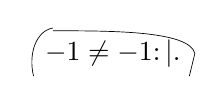
\begin{tikzpicture}
\node[inner sep=3pt] (ineq) {$-1\ne\lVert-1\rVert\unsure{\mathpunct{:}|\mathpunct{.}}$};
\draw[line width=.25pt] ([xshift=-1pt]ineq.south west) .. controls ([xshift=-3pt]ineq.west) and (ineq.north west) .. ([xshift=6pt,yshift=1pt]ineq.north west);
\draw[line width=.25pt] ([xshift=6pt]ineq.north west) .. controls (ineq.north) and (ineq.north east) .. ([xshift=2pt]ineq.east) -- (ineq.south east);
\end{tikzpicture}}
% archive sheet number: 3
\scanpage{5}
\[
L_{\unsure{v|\nu}}(M\otimes T,s)=L_{v}(M)(s\pm1)
\]

\[
\gamma_{\mathbb{R}}(s)\,\gamma_{\mathbb{R}}(s+1)
=\gamma_{\mathbb{C}}\unsure{\mathpunct{:}|\mathpunct{.}}(s)
\]
% archive sheet number: 4
\scanpage{6}
\margin{\tikz[baseline=(eq.base)]{\node[inner sep=3pt] (eq) {$\dfrac{E}{Q}$};\draw[line width=.35pt] (eq.north east) .. controls ([xshift=1pt]eq.east) and (eq.south east) .. (eq.south east) -- ([xshift=-3pt]eq.south west);}}

\diagram{\begin{tikzcd}[ampersand replacement=\&,column sep=.7em,row sep=1em,
execute at end picture={
\draw[line width=.25pt] ([xshift=2pt,yshift=6pt]sa.north west) -- ([xshift=-4pt,yshift=6pt]sa.north west) .. controls (sa.west) and ([xshift=-6pt]ce.west) .. ([xshift=-6pt,yshift=-5pt]ce.south west) -- ([xshift=-1pt,yshift=-5pt]ce.south west);
\draw[line width=.25pt] ([xshift=-1pt,yshift=4pt]sa.north east) -- ([xshift=4pt,yshift=4pt]sa.north east) .. controls ([xshift=6pt]sa.east) and ([xshift=4pt]ce.east) .. ([xshift=7pt,yshift=-4pt]ce.south east) -- ([xshift=0pt,yshift=-5pt]ce.south east);
}]
\& \& \& \& \mathbb{G}_m\,\unsure{\cdot|\mathpunct{.}}\\
E^{*}\arrow[r] \&
{\dfrac{\displaystyle\prod_{E/Q}\mathbb{G}_m}{\overline{U^{\unsure{\wedge|\lambda}}}}} \&
\times \& {\dfrac{I(E)}{I^{\unsure{0|\circ}}(E)}}\arrow[r] \& S_E\arrow[u]\\[-.6em]
\& \& \& \& S_{\unsure{E|\epsilon}}(\unsure{\mathbb{C}|\mathbb{R}})\\[-.6em]
E^{*}\arrow[d,equal] \arrow[r] \& {\text{\uline{$I(E)$}}} \&
\times \& {\dfrac{I(E)}{I^{0}(E)}}\arrow[r] \& |[alias=sa]| S_E(\mathbb{A})\arrow[u]\\
E^{*}\arrow[rr] \& \& I(E)\arrow[ul,"{1}"]\arrow[ur,"{1}"']\arrow[rr] \&
\& |[alias=ce]| {\text{\uuline{$C(E)$}}}\arrow[u]
\end{tikzcd}}
\figure{\begin{tikzpicture}[x=1cm,y=1cm]
\draw[line width=.25pt] (0,0) .. controls (.5,.15) and (1.7,.17) .. (2.7,.17) .. controls (5.5,.35) and (8,.45) .. (10,.42);
\end{tikzpicture}}

\[
\deleted{S_E\longrightarrow\unsure{G|\mathbb{G}}},\qquad
S_E\longrightarrow\mathbb{G}_{m}^{\unsure{h|r_{2}|r}(\unsure{E|K})}
\]
% slanted
\margin{$\unsure{2|\mathbb{Z}}_{\unsure{ve|me|e|\infty}}$}
% archive sheet number: 5
